% Quasi-static PIC on non-uniform radial grids -- draft for Phys. Rev. Accel. Beams
% Compile: pdflatex quarz_paper && pdflatex quarz_paper
\documentclass[aps,prab,reprint,superscriptaddress,amsmath,amssymb]{revtex4-2}

\usepackage{graphicx}
\usepackage{bm}
\usepackage{booktabs}
\usepackage{tikz}
\usetikzlibrary{arrows.meta}
\usepackage[colorlinks=true,linkcolor=blue,citecolor=blue,urlcolor=blue]{hyperref}

\newcommand{\perpv}{\perp}
\newcommand{\dd}{\mathrm{d}}

\begin{document}

\title{Quasi-static particle-in-cell simulation of plasma wakefields\\ on non-uniform radial grids}

\author{Alexander Pukhov}
\author{Thomas C. Wilson}
\affiliation{Institut f\"ur Theoretische Physik I, Heinrich-Heine-Universit\"at D\"usseldorf, 40225 D\"usseldorf, Germany}

\date{\today}

\begin{abstract}
We present a quasi-static particle-in-cell scheme for beam-driven plasma wakefields in $(r,\theta,\xi)$ geometry that works on an arbitrary non-uniform radial grid. The field equations are discretized with hat-function finite elements and conservative finite volumes on any monotone set of radial nodes. The transverse magnetic field is obtained explicitly, without iterations, following Baxevanis and Stupakov. An optional azimuthal mode $m=1$ captures beam offsets, tilts and hosing. The discretization keeps the discrete Gauss law exact, deposits a uniform plasma exactly on every node including the axis, and is second-order accurate on smoothly stretched grids. For a pinched low-emittance witness with mobile ions, a stretched grid of 512 cells ($5\times10^{-4}\,c/\omega_p$ on the axis) gives the near-axis focusing field to 0.03\%, whereas a uniform grid of 1600 cells has a 1.2\% error, at a third of the cost. Both grids converge at second order; for a given accuracy the stretched grid needs about 20 times fewer cells. The scheme is implemented in the C++/Kokkos code QUARZ (Quasistatic Arbitrary-resolution RZ), which runs on CPUs and GPUs and uses MPI with a pipelined decomposition along $\xi$.
\end{abstract}

\maketitle

%---------------------------------------------------------------------------
\section{Introduction}

Quasi-static codes make start-to-end simulations of plasma wakefield accelerators affordable. They exploit the separation of time scales between the plasma response and the evolution of a relativistic driver~\cite{Mora1997}. The plasma is advanced slice by slice in the co-moving variable $\xi = t - z$, and the beam is pushed with a time step set by its betatron period. Established implementations include LCODE~\cite{Lotov2003,Sosedkin2016}, QuickPIC~\cite{Huang2006,An2013}, QPAD~\cite{Li2021}, HiPACE and HiPACE++~\cite{Mehrling2014,Diederichs2022} and Wake-T~\cite{FerranPousa2026}.

Many current problems are strongly multiscale in the radial direction. A low-emittance witness can be focused to a radius of order $10^{-2}\,c/\omega_p$, and it pulls in the plasma ions to densities several times $n_0$ on the axis~\cite{Rosenzweig2005,An2017}. The wake, however, extends over several $c/\omega_p$, and the conducting boundary has to be farther still. A uniform grid must resolve the smallest scale everywhere, so the number of cells, and the cost of each slice, grows with the ratio of the two scales.

Cartesian codes address this with mesh refinement~\cite{Diederichs2022}. In axisymmetric geometry a simpler option is available: a single radial grid with non-uniform spacing, fine on the axis and coarse outside. Ferran Pousa \textit{et al.} recently obtained a similar flexibility in a gridless formulation, by spacing the plasma macro-particles non-uniformly~\cite{FerranPousa2026}. Here we keep a grid, which gives a direct field solve, linear cost in the number of cells, and a natural extension to azimuthal modes.

The contributions of this paper are:
(i) a discretization of the quasi-static field equations on arbitrary radial nodes: hat-function volumes, a lumped-mass finite-element Laplacian for $m=0$ and conservative finite-volume operators for the vector components and for $m=1$ (Sec.~\ref{sec:disc});
(ii) its combination with the explicit, iteration-free $\bm{B}_\perp$ solve of Baxevanis and Stupakov~\cite{Baxevanis2018}, extended to the $m=1$ mode with a short Picard iteration for the mode coupling (Secs.~\ref{sec:model}, \ref{sec:m1});
(iii) exact discrete properties: Gauss law, uniform-plasma deposition including the axis node, and $E_z$ as the exact discrete $\xi$-derivative of $\psi$ (Sec.~\ref{sec:disc});
(iv) a performance-portable implementation with MPI pipelining along $\xi$ (Sec.~\ref{sec:impl}) and a validation set, including a grid study for a pinched witness with ion motion (Sec.~\ref{sec:valid}).

%---------------------------------------------------------------------------
\section{Quasi-static model}\label{sec:model}

We use normalized units: time in $1/\omega_p$, lengths in $c/\omega_p$, densities in $n_0$, momenta in $m_s c$ and fields in $m_e c\,\omega_p/e$. With $\xi = t - z$ and the wake potential $\psi = \phi - A_z$, the transverse force on a particle moving with $v_z = c$ is $\bm{W}_\perp = \bm{E}_\perp + \hat{\bm z}\times\bm{B}_\perp = -\nabla_\perp\psi$. In the quasi-static approximation the fields of one slice follow from the sources of that slice:
\begin{align}
\nabla_\perp^2 \psi &= -(\rho - J_z), \label{eq:psi}\\
\nabla_\perp^2 E_z &= -\partial_\xi(\rho - J_z), \label{eq:ez}\\
\nabla_\perp^2 B_z &= -(\nabla_\perp\times\bm{J}_\perp)_z, \label{eq:bz}\\
\nabla_\perp^2 \bm{B}_\perp &= \hat{\bm z}\times\left(\partial_\xi \bm{J}_\perp - \nabla_\perp J_z\right). \label{eq:bperp}
\end{align}
The term $\partial_\xi\bm{J}_\perp$ is not known on the current slice. Following Baxevanis and Stupakov~\cite{Baxevanis2018}, it is computed from the particle equations of motion. Its part proportional to $\bm{B}_\perp$ is moved to the operator. In complex notation $B_+ = B_x + iB_y$, Eq.~\eqref{eq:bperp} becomes a screened Poisson (Helmholtz) problem,
\begin{align}
\left(\nabla_\perp^2 - \chi\right) B_+ &= i\left[(\partial_x + i\partial_y) J_z + S_+\right], \label{eq:helm}\\
\chi &= \sum_p \frac{q_p^2 w_p}{m_p(\gamma_p - p_{z,p})} \ge 0, \label{eq:chi}
\end{align}
where $S_+$ collects the remaining terms, deposited from the particles. Since $\chi\ge 0$, the operator is negative definite and the solve needs no iteration. Finally $E_+ = W_+ - iB_+$.

\paragraph{Plasma particles} carry $(x, y, p_x, p_y, \Delta = \gamma - p_z, w)$, with $\Delta$ conserved in a static potential. With $\hat q = q/m$ they obey
\begin{align}
\frac{\dd x}{\dd\xi} &= \frac{p_x}{\Delta}, \label{eq:eom}\\
\frac{\dd p_x}{\dd\xi} &= \hat q\left[\frac{\gamma W_x}{\Delta} + B_y + \frac{p_y B_z}{\Delta}\right], \\
\frac{\dd \Delta}{\dd\xi} &= \hat q\left[\frac{\bm{p}_\perp\cdot\bm{W}_\perp}{\Delta} - E_z\right],
\end{align}
and the analogous equations for $y$. They are integrated with an Adams--Bashforth scheme of order 1 to 5 (default 3). Particles are Cartesian in the transverse plane, so they cross the axis without special treatment. Any number of species, including mobile ions, can be used. Particles with $\Delta$ below a threshold are trapped and are removed, since the quasi-static model cannot follow them.

\paragraph{Beam particles} are full 3D macro-particles $(x, y, p_x, p_y, p_z, \xi, w)$, advanced in lab time $t$ with a time step $\Delta t \gg \Delta\xi$. We use the Vay pusher~\cite{Vay2008} by default, because the beam's own fields nearly cancel ($E_r\approx B_\theta$) and the Boris pusher does not preserve this balance; the Higuera--Cary pusher~\cite{Higuera2017} and an implicit scheme with radiation reaction are available. The beam charge and current, $(\rho - J_z)_b$, enter the right-hand sides above.

%---------------------------------------------------------------------------
\section{Discretization on an arbitrary radial grid}\label{sec:disc}

The radial nodes $0 = r_0 < r_1 < \dots < r_N = R$ are arbitrary; $h_j = r_{j+1} - r_j$ and $r_{j+1/2} = (r_j + r_{j+1})/2$. All fields and sources live on the nodes. In practice the grid is built from regions with prescribed spacings, joined geometrically so that the ratio of neighbouring cells stays below a bound (typically 1.05--1.1).

\paragraph{Hat-function volumes.} Charge assignment and field interpolation use the linear hat functions $W_j(r)$ of the non-uniform cells. The volume associated with node $j$ is the exact integral of its hat function,
\begin{align}
V_j &= 2\pi\!\int W_j(r)\,r\,\dd r \nonumber\\
    &= 2\pi\left[\frac{r_{j-1}h_{j-1}}{2} + \frac{h_{j-1}^2}{3} + \frac{r_j h_j}{2} + \frac{h_j^2}{6}\right], \label{eq:vol}
\end{align}
and a density on node $j$ is $\sum_p w_p W_j(r_p)/V_j$. This generalizes Verboncoeur's volume correction~\cite{Verboncoeur2001} to non-uniform cells. Because the volumes are exact, a ring placed at the volume centroid of each radial sub-cell deposits a uniform density exactly on every node, including $r=0$. We load the plasma this way; placing rings at the mid-points instead gives density errors of order 10\% on the axis.

\paragraph{$m=0$ Laplacian.} We use lumped-mass linear finite elements, which with the same $V_j$ coincide with the conservative flux form:
\begin{equation}
(L_0 f)_j = \frac{2\pi}{V_j}\left[r_{j+\frac12}\frac{f_{j+1}-f_j}{h_j} - r_{j-\frac12}\frac{f_j - f_{j-1}}{h_{j-1}}\right]. \label{eq:L0}
\end{equation}
The sum $\sum_j V_j (L_0 f)_j$ telescopes to the flux through the wall, so the discrete Gauss law holds exactly. The axis row contains only the outward flux and needs no regularity condition.

\paragraph{Higher-order operators.} The vector components ($B_+$ modes) and the $m=1$ scalars need $L_n f = (1/r)(r f')' - n^2 f/r^2$ with $n = 1, 2$. We write it in the factorized form $L_n f = r^{n-1}\partial_r\!\left[r^{1-2n}\partial_r(r^n f)\right]$ and discretize it with conservative finite volumes:
\begin{align}
(L_n f)_j &= \frac{2\,r_j^{\,n-1}}{h_{j-1}+h_j}\left(D_{j+1/2} - D_{j-1/2}\right), \label{eq:Ln}\\
D_{j+1/2} &= \frac{r_{j+1}^{\,n} f_{j+1} - r_j^{\,n} f_j}{h_j\, r_{j+1/2}^{\,2n-1}}, \nonumber
\end{align}
with $f(0)=0$. For $n=1$ this is the familiar $\partial_r[(1/r)\partial_r(rB)]$. The factorized form keeps the stencil tridiagonal and well conditioned near the axis on any grid. Each slice therefore requires only tridiagonal solves: Thomas on CPUs and parallel cyclic reduction inside one thread block on GPUs. The $\chi$ term enters the diagonal.

\paragraph{Boundary conditions.} At $r=R$ we impose $\psi = E_z = B_z = 0$ and Dirichlet conditions on $B_r$ and on the $m=1$ parts of $B_+$. For $B_\theta$ we impose the flux condition $(1/r)\partial_r(rB_\theta) = J_z$ at the wall, i.e.\ Amp\`ere's law evaluated at the boundary.

\paragraph{Exact $\xi$-derivatives of the deposits.} The source $\partial_\xi(\rho - J_z)$ of $E_z$, and $\partial_\xi\bm{J}_\perp$, are not differenced between slices. Each particle deposits the exact $\xi$-derivative of its own discrete deposit, $w\,W_j'(r_p)\,\dd r_p/\dd\xi$, plus the azimuthal part for $m=1$. With this choice, $E_z$ is the exact discrete $\xi$-derivative of $\psi$ in every mode.

\paragraph{Gradients} ($\bm{W}_\perp = -\nabla_\perp\psi$ and the Lorentz-force terms) use the three-point second-order formula for non-uniform spacing. On smoothly stretched grids all operators converge at second order; measured orders against manufactured solutions are 1.9--2.0 for $L_0$, $L_1$ and $L_2$ ($h_0 = 0.01\to0.00125$, ratio $\le 1.05$). Abrupt jumps in spacing reduce the accuracy locally to first order.

%---------------------------------------------------------------------------
\section{Azimuthal mode $m=1$}\label{sec:m1}

Every scalar is expanded as $f(r,\theta) = f_0(r) + 2\,\mathrm{Re}[f_1(r)e^{i\theta}]$, as in QPAD~\cite{Li2021} and in quasi-cylindrical electromagnetic codes~\cite{Lifschitz2009}. For transverse vectors it is convenient to expand the complex combination $V_+ = V_x + iV_y$:
\begin{equation}
V_+ = v_0(r) + v_1(r)e^{i\theta} + v_2(r)e^{2i\theta}. \label{eq:vplus}
\end{equation}
Here $v_1 = V_{r0} + iV_{\theta0}$ is the axisymmetric part, while $v_0$ and $v_2$ carry $m=1$. Each coefficient $v_k$ obeys a scalar radial equation with the operator $L_k$ of Sec.~\ref{sec:disc}, so the scalar fields ($\psi$, $E_z$, $B_z$) need $L_0$ and $L_1$, and $B_+$ needs $L_0$, $L_1$ and $L_2$. Regularity on the axis gives $v_1(0) = v_2(0) = 0$.

The only new difficulty is the term $\chi B_+$. With $\chi = \chi_0 + 2\,\mathrm{Re}[\chi_1 e^{i\theta}]$, the product couples $b_k$ to $b_{k\pm1}$. We keep $\chi_0$ in the operator and move the $\chi_1$ products to the right-hand side. A few Picard iterations then converge quickly, because $\chi_1$ is small whenever the $m=1$ description itself is valid; three iterations reached 0.3\% in our tests. For a centred beam the $m=1$ part vanishes identically and the $m=0$ result is recovered to round-off.

Plasma particles stay Cartesian. With $m=1$ every loaded ring is split into $n_\theta$ particles at equidistant azimuths (default 8), and each particle deposits with weights $e^{-ik\theta}$. Beam particles gather the fields as mode sums at their own azimuth. To keep sampling noise from seeding a spurious $m=1$ component, beams can be loaded with an $n$-fold rotational quiet start, or deposited analytically: for a displaced Gaussian the $m=0$ and $m=1$ parts are known in closed form in terms of modified Bessel functions $I_0$, $I_1$.

The expansion is truncated at $m=1$. It therefore describes offsets and tilts that are small compared with the beam and bubble radii, which covers the onset of hosing and beam--plasma misalignment.

%---------------------------------------------------------------------------
\section{Implementation and parallelization}\label{sec:impl}

QUARZ is written in C++17 on Kokkos~\cite{Trott2022}, so one source compiles for OpenMP, CUDA, HIP and SYCL. Particles are stored as structures of arrays, and all particle loops are device kernels with atomic deposition. With $m=0$ a slice costs about 12 kernels and 5 tridiagonal solves; with $m=1$ and three Picard iterations, about 20 kernels and 25 solves. Host--device traffic is limited to loading the fresh plasma slice and to output. The source code of QUARZ, the validation scripts and a first draft of this manuscript were generated with the AI assistant Claude~\cite{Claude} under the direction of the authors (see Acknowledgments).

\paragraph{MPI pipelining along $\xi$.} The box is split into $P$ contiguous blocks of slices, one per rank, with rank 0 at the head. The plasma enters at the head, so rank $r$ can sweep step $n$ only after rank $r-1$ has finished it; but rank $r-1$ can then start step $n+1$ (Fig.~\ref{fig:pipeline}). This time pipelining, used in QuickPIC~\cite{Feng2009} and HiPACE++~\cite{Diederichs2022}, gives a speed-up of $PN/(N+P-1)$ for $N$ sweeps. Once per step, rank $r$ sends rank $r+1$ a single message with: the plasma particles leaving its last slice, with their Adams--Bashforth history; $B_+$ of the last slice, used as the starting guess of the next solve; $(\rho - J_z)_b$ of the last slice, needed for the $\xi$-derivative of the beam source; and beam particles that slipped into the next block during the push ($\dd z/\dd t\le c$, so beam particles only move towards larger $\xi$).

For the pipeline, the beam deposit and the field gather of a slice must not involve slices of another rank at another time level. Beam particles therefore use nearest-slice assignment in $\xi$, with the full hat-function shape in $r$. A serial run with the same assignment performs identical arithmetic, so serial and parallel runs can be compared directly (Sec.~\ref{sec:valid}). On GPUs each rank drives one device and messages pass through host buffers, so no CUDA-aware MPI is needed; the message is small compared with the work of a sweep.

\begin{figure}[t]
\centering
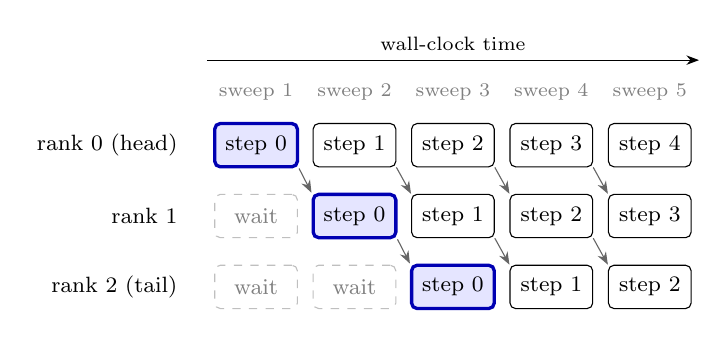
\begin{tikzpicture}[x=1.25cm,y=0.9cm,
  cellbox/.style={draw,rounded corners=2pt,minimum width=1.05cm,minimum height=0.55cm,font=\footnotesize,inner sep=0pt},
  hot/.style={cellbox,very thick,draw=blue!70!black,fill=blue!10},
  idle/.style={cellbox,draw=gray!50,dashed,text=gray},
  msg/.style={-{Stealth[length=1.6mm]},gray!80!black}]
  \foreach \c in {0,...,4} { \node[font=\scriptsize,gray] at (\c,0.75) {sweep \the\numexpr\c+1\relax}; }
  \node[font=\footnotesize,anchor=east] at (-0.7,0)  {rank 0 (head)};
  \node[font=\footnotesize,anchor=east] at (-0.7,-1) {rank 1};
  \node[font=\footnotesize,anchor=east] at (-0.7,-2) {rank 2 (tail)};
  % rank 0
  \node[hot] (a0) at (0,0) {step 0};
  \foreach \c in {1,...,4} { \node[cellbox] (a\c) at (\c,0) {step \c}; }
  % rank 1
  \node[idle] at (0,-1) {wait};
  \node[hot] (b1) at (1,-1) {step 0};
  \foreach \c/\s in {2/1,3/2,4/3} { \node[cellbox] (b\c) at (\c,-1) {step \s}; }
  % rank 2
  \node[idle] at (0,-2) {wait};
  \node[idle] at (1,-2) {wait};
  \node[hot] (c2) at (2,-2) {step 0};
  \foreach \c/\s in {3/1,4/2} { \node[cellbox] (c\c) at (\c,-2) {step \s}; }
  % messages
  \foreach \c/\d in {0/1,1/2,2/3,3/4} { \draw[msg] (a\c.south east) -- (b\d.north west); }
  \foreach \c/\d in {1/2,2/3,3/4} { \draw[msg] (b\c.south east) -- (c\d.north west); }
  \draw[-{Stealth[length=1.6mm]}] (-0.5,1.2) -- (4.5,1.2) node[midway,above,font=\scriptsize] {wall-clock time};
\end{tikzpicture}
\caption{Time pipelining along $\xi$ with three ranks. Arrows: one message per time step from rank $r$ to $r+1$ (plasma particles with their Adams--Bashforth history, $B_+$ and $(\rho-J_z)_b$ of the last slice, and beam particles that slipped downstream). Highlighted: one time step crossing the box. After $P-1$ sweeps all ranks are busy.}
\label{fig:pipeline}
\end{figure}

%---------------------------------------------------------------------------
\section{Validation and benchmarks}\label{sec:valid}

The stretched grid reproduces every reference to the same accuracy as a fine uniform grid, and it is markedly more accurate per cell for near-axis structure. All runs used the OpenMP backend on 2 cores.

\subsection{Verification}

Table~\ref{tab:verif} summarizes the verification tests.

\begin{table*}[t]
\caption{Verification tests (stretched grids have neighbour ratio $\le1.05$).}
\label{tab:verif}
\begin{ruledtabular}
\begin{tabular}{p{0.42\textwidth}p{0.52\textwidth}}
Test & Result \\ \hline
$L_0$, $L_1$, $L_2$ vs manufactured solutions, stretched grids & second order (measured 1.98--2.0) \\
Uniform plasma deposit, stretched grid & exact to $5\times10^{-13}$, including $r=0$ \\
Linear wake ($n_b=10^{-3}$) vs Green's function in a conducting cylinder & $E_z(0)$ error 0.13\% (uniform, 0.01) and 0.12\% (stretched $0.002\to0.05$, 389 cells); the error scales with $n_b$, i.e.\ it is the physical nonlinearity \\
Blowout ($n_b=10$, $\sigma_r=0.3$) & $(E_r-B_\theta)/r = 0.5000$ in the bubble; $E_z$ converged to 4 digits for $\Delta r,\Delta\xi = 0.01\to0.0025$; stretched grid within 0.08\% \\
Betatron oscillation in an ion channel, $\gamma=1000$ & $r_\mathrm{rms}$ follows $r_0|\cos(t/\sqrt{2\gamma})|$ to 0.26\% \\
Witness energy gain, rigid driver & $\dd\langle\gamma\rangle/\dd t = 0.4477$ vs $-E_z = 0.4471$ from the wake \\
Matched witness ($\sigma_r=0.01$, $\varepsilon_n=0.01$, $\gamma=2\times10^4$), $400/\omega_p$ & $\varepsilon_n$ preserved ($0.0097\to0.0097$) for $\Delta t = 10$ and 20; Boris: 9\% spurious growth \\
$m=1$: displaced driver ($d=0.01$, linear regime) vs $-d\,\partial_r$ of the $m=0$ solution & L2 errors $\psi$ 0.08\%, $E_z$ 0.4\%, $E_r$ 0.3\%, $B_\theta$ 0.19\%; sine parts $\le 6\times10^{-14}$ \\
$m=1$: offset beam ($x_0=0.05$) in an ion channel & centroid follows $x_0\cos(t/\sqrt{2\gamma})$ to 0.26\% \\
\end{tabular}
\end{ruledtabular}
\end{table*}

\subsection{Pinched witness with ion motion}\label{sec:pinch}

This is the case the non-uniform grid is designed for. A Gaussian driver ($n_b=10$, $\sigma_r=0.3$, $\sigma_\xi=1$) drives a blowout in a hydrogen plasma column of radius 7 inside a conducting wall at $R=8$. A witness with peak density $1.25\times10^4$, $\sigma_r=0.01$ and $\sigma_\xi=0.1$ (matched for $\varepsilon_n=0.01$ at $\gamma=2\times10^4$) sits at $\xi=6.8$ and pulls the ions onto the axis (Fig.~\ref{fig:maps}). Within the witness the ion density on the axis rises to $2.3\,n_0$, and the focusing gradient at $r=0.01$ is 0.88 instead of the 0.5 of an unperturbed ion column.

\begin{figure*}[t]
\centering
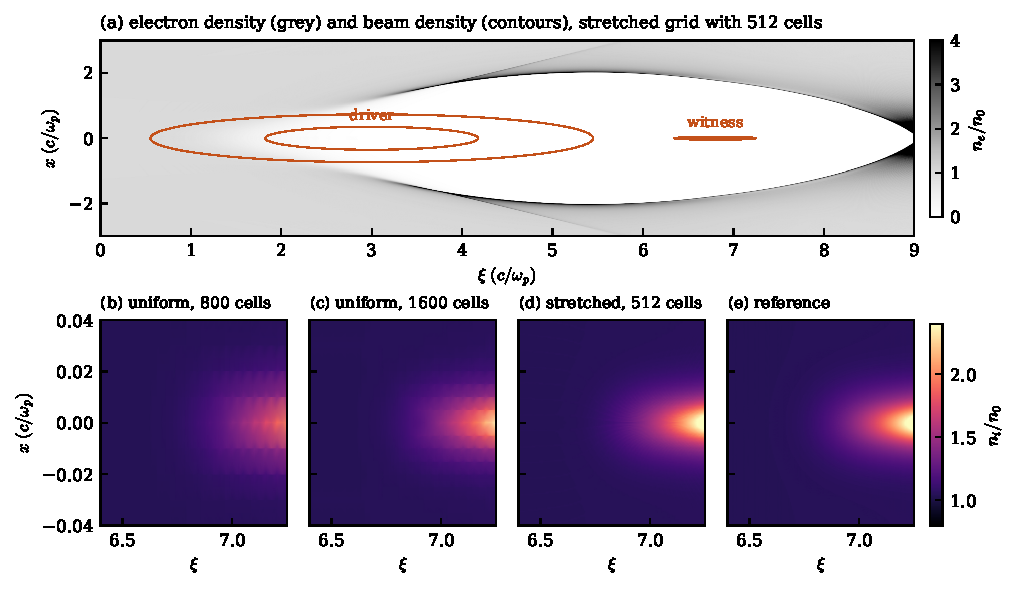
\includegraphics[width=\textwidth]{figs/fig_maps.pdf}
\caption{Pinched witness with mobile hydrogen ions (single quasi-static solve, noise-free beams). (a) Electron density and beam density contours over the whole box, stretched grid with 512 cells. (b)--(e) Ion density near the axis inside the witness: uniform grids with $\Delta r = 0.01$ (800 cells) and $0.005$ (1600 cells), the stretched grid of (a) with $h_0 = 5\times10^{-4}$ on the axis, and the reference ($h_0 = 1.6\times10^{-5}$, 14\,617 cells). On the uniform grids the ion spike is spread over the first cells and its peak is too low; the stretched grid is indistinguishable from the reference.}
\label{fig:maps}
\end{figure*}

To separate grid errors from sampling noise, both beams are deposited analytically in this test (Sec.~\ref{sec:m1}), and we compare one quasi-static solve on a sequence of grids. The uniform family has $\Delta r = 0.02\ldots0.00125$ (400 to 6400 cells). The stretched family scales all three spacings of the 512-cell grid ($5\times10^{-4}$ for $r<0.05$, $0.01$ for $r<2.5$, $0.05$ outside, ratio $\le 1.05$) by factors 4 to 1/8 (172 to 3697 cells). The reference is the same stretched family at factor 1/32 (14\,617 cells). It agrees with a uniform grid of 32\,000 cells ($\Delta r = 2.5\times10^{-4}$) to $2\times10^{-4}$, the accuracy of that uniform grid. All runs use $\Delta\xi = 0.005$. Errors are maxima over the witness ($6.4<\xi<7.2$), relative to the maximum of the reference.

\begin{figure*}[t]
\centering
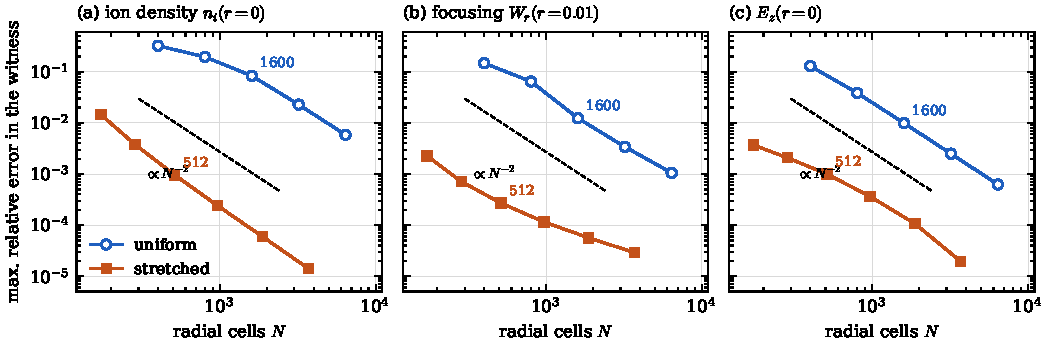
\includegraphics[width=\textwidth]{figs/fig_convergence.pdf}
\caption{Error versus number of radial cells for the pinched witness of Fig.~\ref{fig:maps}: (a) ion density on the axis, (b) focusing field $W_r = E_r - B_\theta$ at $r=0.01$ (the witness radius), (c) $E_z$ on the axis. Open circles: uniform grids; squares: stretched grids with the same shape and all spacings scaled. The grids of Table~\ref{tab:pinch} are labelled. The flattening of the finest stretched points in (b) reflects the accuracy of the reference.}
\label{fig:convergence}
\end{figure*}

Figure~\ref{fig:convergence} shows that both families converge at second order, as expected from Sec.~\ref{sec:disc}, but the stretched curves lie one to two orders of magnitude lower. To reach $10^{-3}$ in the focusing field, the uniform grid needs 6400 cells (15.2~s per sweep), the stretched grid fewer than 300 (0.9~s per sweep): 20 times fewer cells and 17 times less time. Table~\ref{tab:pinch} lists the grids of Fig.~\ref{fig:maps}. With a third of the cells and a third of the time of the 1600-cell uniform grid, the 512-cell stretched grid is 10 times more accurate in $E_z$ and 45--90 times more accurate in the ion density and the focusing field.

\begin{table*}[t]
\caption{Pinched witness with mobile hydrogen ions: maximum relative errors in the witness with respect to the reference of Fig.~\ref{fig:convergence}. $W_r = E_r - B_\theta$. Times per sweep of 1461 slices on 2 CPU cores.}
\label{tab:pinch}
\begin{ruledtabular}
\begin{tabular}{lrrrrrr}
Grid & cells & time per sweep (s) & $n_i(0)$ & $W_r(0.01)$ & $W_r(0.03)$ & $E_z(0)$ \\ \hline
uniform 0.01 & 800 & 2.0 & 20\% & 6.5\% & 3.0\% & 3.9\% \\
uniform 0.005 & 1600 & 4.1 & 8.4\% & 1.2\% & 0.83\% & 0.99\% \\
stretched $0.0005\to0.01\to0.05$ & 512 & 1.4 & 0.10\% & 0.027\% & 0.015\% & 0.10\% \\
\end{tabular}
\end{ruledtabular}
\end{table*}

With randomly sampled macro-particle beams ($4\times10^5$ driver and $2\times10^5$ witness particles) the errors of the 512-cell stretched grid rise to 0.3\% in $W_r(0.01)$ and 5\% in $n_i(0)$. They are then set by beam sampling noise, not by the grid: fine cells near the axis must be paired with enough beam particles there, or with a quiet start.

\paragraph*{Witness evolution.} The field errors carry over into the beam dynamics. Figure~\ref{fig:evolution} follows the witness ($2\times10^5$ macro-particles) for 100 steps of $\Delta t = 10$, behind a rigid, analytically deposited driver, so that only the witness, the plasma electrons and the ions evolve. The witness was matched to the unperturbed ion column; the collapsed ions focus it more strongly, so its rms radius oscillates. On the 800- and 1600-cell uniform grids the first minimum of $r_\mathrm{rms}$ is 3.7\% and 2.7\% below the initial value, i.e.\ the amplitude is overestimated by 64\% and 16\%. The 512-cell stretched grid gives 2.29\%, within 0.1\% of the amplitude on a stretched grid twice as fine (967 cells); its sweep is 3 times faster than that of the 1600-cell uniform grid. The emittance oscillates by only 0.16\% in all runs. The energy gain over the run, $\Delta\gamma\approx 329$, is 1.2\% and 0.3\% too low on the uniform grids and within 0.07\% on the 512-cell stretched grid.

\begin{figure*}[t]
\centering
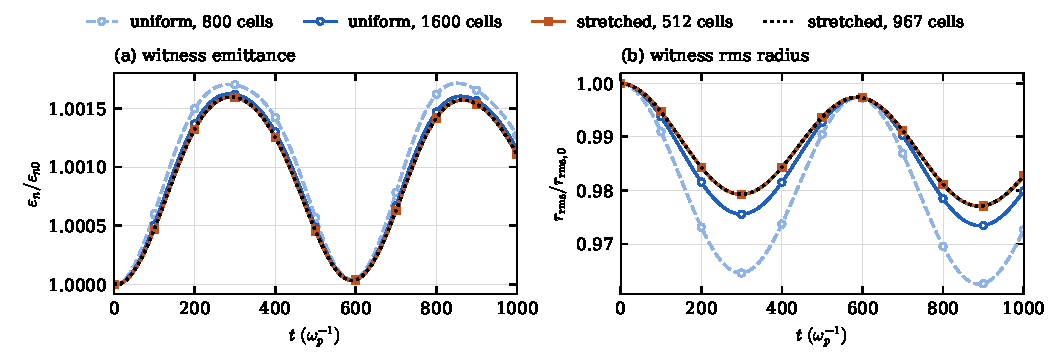
\includegraphics[width=\textwidth]{figs/fig_evolution.pdf}
\caption{Evolution of the pinched witness of Fig.~\ref{fig:maps} behind a rigid driver, with mobile hydrogen ions, on two uniform and two stretched grids ($\Delta t = 10$, $2\times10^5$ witness particles). (a) Normalized emittance, (b) rms radius, both relative to their initial values. The 512-cell stretched grid coincides with the 967-cell one; the uniform grids overestimate the envelope oscillation.}
\label{fig:evolution}
\end{figure*}

\subsection{Parallel runs}

MPI runs were compared file by file with serial runs that use the same nearest-slice beam assignment. Runs without beam particles crossing rank boundaries are bit-identical (witness gain, ion motion, parsed profiles, analytic offset driver with $m=1$). When particles move between ranks, their order in memory changes and the results differ at round-off level: $10^{-10}$ in the fields for hosing ($m=1$, 12 steps) and $5\times10^{-8}$ for a $\gamma=5$ beam slipping through all ranks. On 2 CPU cores the speed-up is 1.77--1.83 for 13--25 sweeps, against 1.86--1.92 for an ideal pipeline. GPU performance has not yet been measured.

%---------------------------------------------------------------------------
\section{Conclusions}

A quasi-static RZ scheme can run on any monotone radial grid without losing the properties that make uniform-grid codes robust: exact discrete Gauss law, exact uniform-plasma deposition on the axis, second-order accuracy and an iteration-free $\bm{B}_\perp$ solve. The cost per slice stays linear in the number of cells, so resolution can be spent where the physics needs it. For a pinched witness with ion motion this gives 10--90 times smaller errors than a uniform grid at a third of the cost, or the same accuracy with 20 times fewer cells. The same operators carry over to the $m=1$ mode, and the code scales across CPU cores and GPUs through pipelining along $\xi$.

Natural extensions are a laser envelope solver on the same grid (a complex tridiagonal Crank--Nicolson step per slice), higher azimuthal modes, and adaptive grids that follow the witness radius during the run.

%---------------------------------------------------------------------------
\begin{acknowledgments}
The QUARZ source code, its validation suite, the simulations and figures of Sec.~\ref{sec:valid}, and a first draft of this manuscript were produced with the large language model Claude (Anthropic; model identifier \texttt{claude-opus-5-5})~\cite{Claude}, working under the direction of A.P. T.C.W. tested the code. The authors reviewed and edited the text and take full responsibility for the content of this article. Claude is not an author, because it cannot take responsibility for the work.
\end{acknowledgments}

\begin{thebibliography}{99}
\bibitem{Mora1997} P. Mora and T. M. Antonsen, Jr., Kinetic modeling of intense, short laser pulses propagating in tenuous plasmas, Phys. Plasmas \textbf{4}, 217 (1997).
\bibitem{Lotov2003} K. V. Lotov, Fine wakefield structure in the blowout regime of plasma wakefield accelerators, \href{https://doi.org/10.1103/PhysRevSTAB.6.061301}{Phys. Rev. ST Accel. Beams \textbf{6}, 061301 (2003)}.
\bibitem{Sosedkin2016} A. P. Sosedkin and K. V. Lotov, LCODE: A parallel quasistatic code for computationally heavy problems of plasma wakefield acceleration, Nucl. Instrum. Methods Phys. Res., Sect. A \textbf{829}, 350 (2016).
\bibitem{Huang2006} C. Huang \textit{et al.}, QUICKPIC: A highly efficient particle-in-cell code for modeling wakefield acceleration in plasmas, J. Comput. Phys. \textbf{217}, 658 (2006).
\bibitem{An2013} W. An \textit{et al.}, An improved iteration loop for the three dimensional quasi-static particle-in-cell algorithm: QuickPIC, J. Comput. Phys. \textbf{250}, 165 (2013).
\bibitem{Li2021} F. Li \textit{et al.}, A quasi-static particle-in-cell algorithm based on an azimuthal Fourier decomposition for highly efficient simulations of plasma-based acceleration: QPAD, Comput. Phys. Commun. \textbf{261}, 107784 (2021).
\bibitem{Mehrling2014} T. Mehrling \textit{et al.}, HiPACE: a quasi-static particle-in-cell code, Plasma Phys. Control. Fusion \textbf{56}, 084012 (2014).
\bibitem{Diederichs2022} S. Diederichs \textit{et al.}, HiPACE++: A portable, 3D quasi-static particle-in-cell code, Comput. Phys. Commun. \textbf{278}, 108421 (2022).
\bibitem{FerranPousa2026} A. Ferran Pousa \textit{et al.}, Gridless quasistatic model for efficient simulation of plasma-based accelerators, \href{https://arxiv.org/abs/2603.16623}{arXiv:2603.16623 (2026)}.
\bibitem{Rosenzweig2005} J. B. Rosenzweig \textit{et al.}, Effects of ion motion in intense beam-driven plasma wakefield accelerators, Phys. Rev. Lett. \textbf{95}, 195002 (2005).
\bibitem{An2017} W. An \textit{et al.}, Ion motion induced emittance growth of matched electron beams in plasma wakefields, Phys. Rev. Lett. \textbf{118}, 244801 (2017).
\bibitem{Baxevanis2018} P. Baxevanis and G. Stupakov, Novel fast simulation technique for axisymmetric plasma-wakefield acceleration configurations in the blowout regime, \href{https://doi.org/10.1103/PhysRevAccelBeams.21.071301}{Phys. Rev. Accel. Beams \textbf{21}, 071301 (2018)}.
\bibitem{Vay2008} J.-L. Vay, Simulation of beams or plasmas crossing at relativistic velocity, Phys. Plasmas \textbf{15}, 056701 (2008).
\bibitem{Higuera2017} A. V. Higuera and J. R. Cary, Structure-preserving second-order integration of relativistic charged particle trajectories in electromagnetic fields, Phys. Plasmas \textbf{24}, 052104 (2017).
\bibitem{Verboncoeur2001} J. P. Verboncoeur, Symmetric spline weighting for charge and current density in particle simulation, J. Comput. Phys. \textbf{174}, 421 (2001).
\bibitem{Lifschitz2009} A. F. Lifschitz \textit{et al.}, Particle-in-cell modelling of laser--plasma interaction using Fourier decomposition, J. Comput. Phys. \textbf{228}, 1803 (2009).
\bibitem{Trott2022} C. R. Trott \textit{et al.}, Kokkos 3: Programming model extensions for the exascale era, IEEE Trans. Parallel Distrib. Syst. \textbf{33}, 805 (2022).
\bibitem{Claude} Anthropic, Claude, large language model (model \texttt{claude-opus-5-5}), \url{https://www.anthropic.com/claude}, used in October 2026.
\bibitem{Feng2009} B. Feng \textit{et al.}, Enhancing parallel quasi-static particle-in-cell simulations with a pipelining algorithm, J. Comput. Phys. \textbf{228}, 5340 (2009).
\end{thebibliography}

\end{document}
